\section{Graphentheorie}
Mathematiker lieben es Probleme zu verallgemeinern. Um den Vier-Farben-Satz in ein Format zu bringen, mit dem gearbeitet werden kann, kann man jede Fläche einer Karte als einen Punkt (fachsprachlich: Knotenpunkt) auf einem planaren Graphen (planar bedeutet, dass sich keine Kante mit einer anderen schneidet) und jede Berührung zwischen jeder Fläche mit einer Linie (fachsprachlich: Kante) darstellen. Das macht es einfacher, denn somit werden Karten, die verschieden aussehen aber in der Graphentheorie an sich gleich sind, auch gleich dargestellt. Dadurch kann das Problem allgemeiner formuliert werden. Aus \textit{"Flächen, bei denen sich die gleichen Farben nicht berühren dürfen"} wird \textit{"Knoten, die nicht mit anderen gleichfarbigen Knoten verbunden werden dürfen"}. Im Allgemeinen lässt sich hier auch die Verbindung zu den Kameras und Stundenplänen ziehen, man bildet Knoten für jedes Objekt, verbietet bestimmte Arten von Verbindungen zwischen diesen Knoten und muss mit diesen Limitationen auf das effizienteste Ergebnis kommen. 

\begin{center}
    \begin{tikzpicture}
        \draw[fill=yellow!60] (0,0) -- (90:2) arc (90:90+120:2) -- (0,0);
        \draw[fill=blue!60] (0,0) -- (90+120:2) arc (90+120:90+120+120:2) -- (0,0);
        \draw[fill=red!60] (0,0) -- (90+120+120:2) arc (90+120+120:90+120+120+120:2) -- (0,0);
        \draw[fill=turquoise!60] (0,0) circle (0.5);
    
        \node[circle, draw=black, fill=yellow] (v1) at (120+30:1.35) {};
        \node[circle, draw=black, fill=blue] (v2) at (240+30:1.35) {};
        \node[circle, draw=black, fill=red] (v3) at (0+30:1.35) {};
        \node[circle, draw=black, fill=turquoise] (v4) at (0,0) {};
        
        \draw[] (v1) -- (v2) -- (v3) -- (v4) -- (v2);
        \draw[] (v4) -- (v1) -- (v3);
    \end{tikzpicture}
\end{center}

\subsection{Der Eulersche Polyedersatz}
\begin{center}
    \textit{Sei $E$ die Anzahl der Ecken (Knoten), $K$ die Anzahl der Kanten und $F$ die Anzahl der Flächen. Dann gilt für jeden planaren Graphen $E-K+F=2$.}
\end{center}
Der Satz leitet sich eigentlich aus konvexen Körpern (Körper, die keine ``Einbuchtungen`` oder ``Aushöhlungen`` haben) hervor, aber da jeder konvexe Körper als planarer Graph dargestellt werden kann, passt dies wunderbar für unser Problem. Zufälligerweise ist unser planarer Graph genau der einer dreiseitigen Pyramide (Tetraeder). Man kann den Polyedersatz an unserem Beispiel anwenden und überprüfen, ob er stimmt:

\begin{center}
    \begin{tikzpicture}
        \fill[fill=yellow!50] (240+30:1.5) -- (0+30:1.5) -- (0,0);
        
        \node[circle, draw=black, fill=yellow] (v1) at (120+30:1.5) {};
        \node[circle, draw=black, fill=blue] (v2) at (240+30:1.5) {};
        \node[circle, draw=black, fill=red] (v3) at (0+30:1.5) {};
        \node[circle, draw=black, fill=turquoise] (v4) at (0,0) {};
        \draw[] (v1) -- (v2) -- (v3) -- (v1);
        \foreach \x in {1,2,3}
            \draw[] (v4) -- (v\x);
        
        \node[rectangle, draw=black] (Knoten) at (90:1.5) {Ecke/Knoten};
        \node[rectangle, draw=black] (Fläche) at (330:2.5) {Fläche};
        \node[rectangle, draw=black] (Kante) at (330-120:2.5) {Kante};
        \draw[->] (Knoten) -- (v1);
        \draw[->] (Fläche) -- (330:0.5);
        \draw[->] (Kante) -- (330-120:0.75);
    \end{tikzpicture}
    \[E=4,K=6,F=4\]
\end{center}

Damit wird aus $E-K+F=2$ dann $4-6+4=2$. Wichtig: Der Platz um den Graphen herum zählt auch als Fläche. Somit trifft dieser zu. Dies kann man für jeden beliebigen planaren Graphen wiederholen, das Ergebnis wird immer zwei sein. Als simples Beispiel:

\begin{center}
    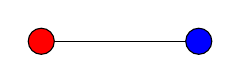
\begin{tikzpicture}
        \node[circle, draw=black, fill=red] (v1) at (0,0) {};
        \node[circle, draw=black, fill=blue] (v2) at (2,0) {};
        \draw[] (v1) -- (v2);
    \end{tikzpicture}
    \[E=2,K=1,F=1\]
    \[E-K+F=2-1+1=2\]
\end{center}

Ein etwas größeres Beispiel:

\begin{center}
    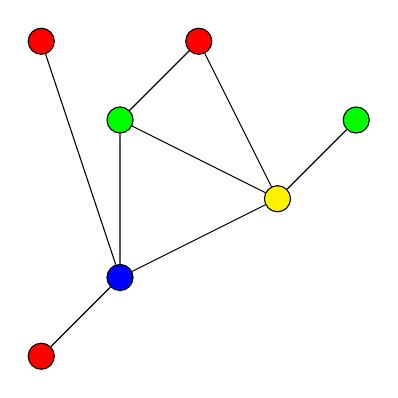
\begin{tikzpicture}
        \node[circle, draw=black, fill=red] (v1) at (0,-1) {};
        \node[circle, draw=black, fill=blue] (v2) at (1,0) {};
        \node[circle, draw=black, fill=yellow] (v3) at (3,1) {};
        \node[circle, draw=black, fill=green] (v4) at (4,2) {};
        \node[circle, draw=black, fill=red] (v5) at (2,3) {};
        \node[circle, draw=black, fill=red] (v6) at (0,3) {};
        \node[circle, draw=black, fill=green] (v7) at (1,2) {};
        \draw[] (v1) -- (v2) -- (v3) -- (v5)
        (v2) -- (v6)
        (v2) -- (v7) -- (v5)
        (v7) -- (v3) -- (v4);
    \end{tikzpicture}
    \[E=7,K=8,F=3\]
    \[E-K+F=7-8+3=2\]
\end{center}

\subsection{Fünf Nachbarn oder weniger}
Damit der Sechs- und Fünf-Farben-Satz bewiesen werden kann, muss eine wichtige Feststellung gemacht werden: Auf jedem planaren Graphen befindet sich mindestens ein Punkt mit fünf oder weniger Verbindungen. Da dies ein fundamentaler Bestandteil unserer Beweise sein wird, folgt hier der Beweis.
\begin{theorem}
    Jeder planare Graph besitzt einen Knotenpunkt mit fünf oder weniger Verbindungen.
\end{theorem}
\begin{proof}
    Es wird ein Beweis durch Widerspruch durchgeführt. Wenn angenommen wird, dass es auf einem planaren Graphen für jeden Knotenpunkt sechs oder mehr Nachbarn gibt, dann gilt $2K \geq 6E \Rightarrow E \leq \frac{1}{3}K $, da eine Verbindung immer zwei Enden hat bzw. zwei Knoten verbindet. Grundlegend gilt für Graphen mit mehr als einer Kante, dass jede Fläche mindestens drei Seiten besitzt und jede Seite an maximal zwei Flächen grenzt. $3F \leq 2K \Rightarrow F \leq \frac{2}{3}K$. Nun gibt es neue Wege um $E$ und $F$ darzustellen, man kann diese in den Eulerschen Polyedersatz einfügen.
    \begin{gather*}
        2=E-K+F\\
        E{\leq \color{blue}\frac{1}{3}K} \quad \textrm{und} \quad F{\leq \color{blue}\frac{2}{3}K}\\
        \Rightarrow \quad {\color{red} 2}=E-K+F {\color{red} \leq}{\color{blue}\frac{1}{3}K}-K+{\color{blue}\frac{2}{3}K} = {\color{red} 0}
    \end{gather*}
    
    Alles wurde unter Annahme, dass alle Knoten mehr als 5 Nachbarn besitzen, hergeleitet, daher müssen alle Schritte stimmen. Aber es läuft auf $2 \leq 0$ hinaus, was eindeutig ein Widerspruch ist. Das bedeutet, dass die Annahme, dass alle Knoten mehr als 5 Nachbarn besitzen, falsch sein muss.
\end{proof}